\documentclass{MO824}
\usepackage[utf8]{inputenc}
\usepackage[brazil]{babel}      % para texto em Português
\usepackage{amsfonts}
\usepackage{amsmath,amssymb}
\usepackage{graphicx}
\usepackage{xcolor}
\usepackage{hyperref}
\usepackage{multirow}
\usepackage{algorithmic}
\usepackage{subfig}
\usepackage{float}
\usepackage[ruled, vlined, portuguese]{algorithm2e}
\newcommand{\Z}{\mathbb{Z}}
\newcommand{\B}{\mathbb{B}}
\newcommand{\N}{\mathbb{N}}
\newcommand{\R}{\mathbb{R}}

\title{Atividade 8 - Grupo 4 - MO824}

\author{
    Victor Ferreira Ferrari      - RA 187890\\
    Luma Gabino Vasconcelos      - RA 202495 \\
    Guilherme de Oliveira Macedo - RA 208395
}

\begin{document}

\criartitulo

\runningheads{V.F. Ferrari, L.G. Vasconcelos e G.d.O. Macedo}%
{Atividade 8}

\begin{abstract}
{\bf Resumo}. Este trabalho apresenta avaliações de desempenho de três metaheurísticas para o problema MAX-QBFPT, além da resolução de dois modelos matemáticos distintos pelo \textit{software} Gurobi, por \textit{TTT Plots} (apenas as metaheurísticas) e Perfis de Desempenho, junto com uma justificativa matemática por trás de cada método. As metaheurísticas testadas foram GRASP, Busca Tabu e Algoritmo Genético. Os resultados indicam que os métodos, em geral, não seguem distribuições exponenciais deslocadas, com exceção do Algoritmo Genético, e um destaque para a Busca Tabu por conseguir ótimos resultados de modo eficiente, em menos tempo que os outros métodos.

{\bf Palavras-chave}. Otimização, Desempenho, ttt-plots, performance profiles, QBFPT, QBF, metaheurísticas.

\end{abstract}

\section{Introdução}
    \paragraph*{}
    Este trabalho consiste na análise de desempenho de soluções exatas e heurísticas, baseada nos métodos de perfis de desempenho e \textit{ttt-plots}, para o problema MAX-QBF com triplas proibidas, proposto na Atividade 8 de MO824 2S-2020. 
    
    O Problema MAX-QBF com Triplas Proibidas (MAX-QBFPT) é uma variação do Problema  MAX-QBF (``\textit{Maximum Quadractic Binary Function}''), em que se objetiva maximizar uma função binária quadrática, de modo que $x_i$, $x_j$ e $x_k$ não assumam o valor 1 simultaneamente caso ($i$, $j$, $k$) forme uma tripla proibida. 
    
    \subsection{Modelo Matemático}
    Uma QBF é uma função binária quadrática $f:\B^n \rightarrow \R$ que pode ser expressa como uma soma de termos quadráticos utilizando variáveis binárias. Sejam~$a_{ij} \in \mathbb{R}$ $(i,j = 1,\dots,n)$ os coeficientes de $f$, no problema em que estamos interessados, uma QBF é dada por:
    
    \begin{equation}\label{qbf}
		f(x_1,...,x_n) = \sum_{i=1}^{n} \sum_{j=1}^{n} a_{ij} \cdot x_{i} \cdot x_{j}
	\end{equation}
    
    Sejam $x_i$ as variáveis binárias de uma QBF $f(x_1, \dots, x_n)$, para $i \in \{1 \dots n\}$ e $\mathcal{T} = \{(i,j,k)\in \N : 1 \leq i < j < k \leq n\}$ o conjunto de todas as triplas ordenadas, sem repetição, dos naturais de 1 a $n$. Dado um conjunto de triplas proibidas $T \subseteq \mathcal{T}$, o problema MAX-QBFPT consiste na maximização de $f(x_1, \dots, x_n)$, de modo que $x_i$, $x_j$ e $x_k$ não sejam todos iguais a 1, para cada $(i, j, k) \in T$. Com base nisso, o MAX-QBFPT pode ser formulado como segue:
    
    \begin{minipage}{\linewidth}
		\begin{flalign}\notag
		&& \max Z = \sum_{i=1}^{n} \sum_{j=1}^{n} a_{ij} \cdot x_i \cdot x_j &&\\
		\label{orig_ineq_01}
		&& \text{s.a} \phantom{aaaa} x_i + x_j + x_k \leq  2, && \forall (i, j, k) \in T 			 \\
		\label{orig_ineq_02}
		&& x_i \in \mathbb{B}.          && \forall i \in \{1,...,n\} 
		\end{flalign}~
	\end{minipage}
    
    As restrições \eqref{orig_ineq_01} correspondem às restrições das triplas proibidas, isto é, impedem que toda solução contenha um subconjunto qualquer de triplas ordenadas sem repetições e proibidas. As restrições \eqref{orig_ineq_02} impõem o domínio das variáveis de decisão como sendo binárias. A função objetivo maximiza o valor da QBF.

    \subsection{Linearização com Triplas Proibidas}
    Para a linearização do problema MAX-QBF com triplas proibidas, utilizamos a seguinte formulação:
    
    \begin{minipage}{\linewidth}
    	\begin{flalign}\notag
    	&& \max Z = \sum_{i=1}^{n} \sum_{j=1}^{n} a_{ij} \cdot x_i \cdot x_j &&\\
    	\label{ineq_01}
    	&& \text{s.a} \phantom{aaaa} x_i + x_j + x_k \leq  2, && \forall (i, j, k) \in T 			 \\
    	\label{ineq_02}
    	&& w_{ij}  \leq x_i && \forall i \in \{1,...,n\} , \forall j = \{1,...,n\}		 \\
    	\label{ineq_03}
    	&& w_{ij}  \leq x_j && \forall i \in \{1,...,n\} , \forall j = ]\{1,...,n\}		 \\
    	\label{ineq_04}
    	&& w_{ij}  \geq x_i + x_j - 1 && \forall i \in \{1,...,n\} , \forall j = \{1,...,n\}		 \\
    	\label{ineq_05}
    	&& x_i \in \mathbb{B}.          && \forall i \in \{1,...,n\}  \\
    	\label{ineq_06}
    	&& w_{ij} \geq 0        && \forall i \in \{1,...,n\} , \forall j = \{1,...,n\}		
    	\end{flalign}~
    \end{minipage}

    
    \subsection{Conjunto de Triplas Proibidas}
    
    Especificamente para esta atividade, as triplas são geradas a partir de duas funções $g,h : [1, n] \rightarrow [1, n]$, que são definidas do seguinte modo:
    
    
    \begin{equation*}
    l_1(u) = 1 + ((\beta_1 \cdot (u - 1) + \beta_2 ) \; mod \; n) 
    \end{equation*}
    
    
    \begin{equation*}
    g(u) = \begin{cases} l_1(u), & \mbox{se } l_1(u) \neq u \\
                        1 + (l_1(u) \; mod \; n), & \mbox{caso contrário } \end{cases}
    \end{equation*}
    
    \begin{equation*}
    l_2(u) = 1 + ((\pi_1 \cdot (u - 1) + \pi_2 ) \; mod \; n) 
    \end{equation*}
    
    
    \begin{equation*}
    h(u) = \begin{cases} l_2(u), & \mbox{se } l_2(u) \neq u  \mbox{ e } l_2(u) \neq g(u)\\
                        1 + (l_2(u) \; mod \; n), & \mbox{se } (1+(l_2(u) \; mod \; n)) \neq u  \mbox{ e } \\ & ~~~~(1+(l_2(u) \; mod \; n)) \neq g(u)\\
                        1 + ((l_2(u)+1) \; mod \; n), & \mbox{caso contrário } \end{cases}
    \end{equation*}

    Onde os valores de $\beta_1$, $\beta_2$, $\pi_1$ e $\pi_2$ são respectivamente 131, 1031, 193 e 1093.
    
    A partir dessas funções definimos o conjunto de triplas proibidas como $T = \{(i,j,k)\in \mathcal{T} : 
    \forall u \in [1,n],  (i,j,k) = sort(\{u, g(u), h(u)\})\}$.

\section{Metodologia} \label{method}
Para a avaliação, foram escolhidas versões de três metaheurísticas diferentes: GRASP, Busca Tabu e Algoritmos Genéticos, assim como implementações dos dois modelos apresentados na seção anterior. As implementações das metaheurísticas foram escolhidas por meio da qualidade dos resultados obtidos em seus respectivos testes.

\subsection{GRASP} \label{grasp}
O GRASP é uma metaheurística que possui duas fases por iteração, sendo elas a construção e a busca local. A fase de construção, juntamente com a função que faz o reparo da solução, é responsável por gerar uma solução viável para o problema, por meio de uma heurística gulosa aleatorizada. Já a fase de busca local consiste em, a partir desta solução, varrer a vizinhança em busca de uma solução melhor. Por último, a melhor solução encontrada é atualizada, se necessário. Como critério de parada, o GRASP possui um número máximo de execuções e tempo limite.

% \vspace{-0.18cm}
% \begin{algorithm}[H]
% 	\label{alg_grasp}
% 	\caption{GRASP(Max\textunderscore Iterations, Seed, $\alpha$)}
% 	\begin{algorithmic}[1]
% 	    \STATE Read.Input();
% 	    \FOR {$k$ = 1,...,Max\textunderscore Iterations}
% 	        \STATE {Solution $\leftarrow$  Greedy\textunderscore Randomized\textunderscore Contruction(Seed, $\alpha$);}\\
% 	        \IF {Solution \emph{is not feasible}} 
% 	            \STATE {Solution $\leftarrow$ Repair(Solution);} \\
% 	       \ENDIF
%                 \STATE {Solution $\leftarrow$ Local\textunderscore Search(Solution);} \\
%                 \STATE {Update\textunderscore Solution(Solution, Best\textunderscore Solution);} \\
% 	  \ENDFOR
% 	  \RETURN  Best\textunderscore Solution;
% 	\end{algorithmic}
% \end{algorithm}
%\vspace{0.5cm}

O método de construção utilizado foi o Cost Perturbations, no qual a ideia principal é introduzir algum ruído nos custos originais. Essa abordagem incorpora mecanismos de aprendizagem associados a estratégias de intensificação e diversificação. O hiperparâmetro foi fixado em $\alpha=0.4$. Note que esse método elimina a aleatoriedade da heurística construtiva.

\subsection{Busca Tabu} \label{tabu}
A Busca Tabu é uma meta-heurística baseada em busca local que surgiu da ideia de utilizar uma \textbf{memória} para superar ótimos locais. A técnica permite a realização de movimentos que não melhoram a solução atual, evitando ciclos por meio de memórias chamadas de \textbf{listas tabu}. Uma lista tabu é uma estrutura de dados responsável por armazenar os últimos movimentos aplicados por um determinado número de iterações, a fim de evitar que eles sejam desfeitos por novos movimentos. Assim, uma descrição básica do método consiste em construir uma solução inicial e realizar iterativamente um movimento de vizinhança que não seja proibido, guardando-o na lista tabu.

O algoritmo básico consiste da construção de uma solução inicial (gulosa), seguida de uma série de movimentos de vizinhança, atualizando a melhor solução a cada iteração e adicionando cada movimento na lista tabu (removendo a entrada mais antiga, caso necessário).

% \vspace{-0.18cm}
% \begin{algorithm}[H]
%     \label{alg_tabu_search}
%     \caption{BuscaTabu (maxIteracoes, tenure, maxTempo)}
% 	\begin{algorithmic}[1]
% 		\STATE $x^{*} \leftarrow x_{0}$; \COMMENT{Solução inicial}
% 		\STATE $T \leftarrow \emptyset$; \COMMENT{Lista tabu}
% 		\WHILE{iteracaoAtual < maxIteracoes \AND tempo < maxTempo}
% 		    \STATE Seja $x' \leftarrow x \oplus m$ o melhor elemento de $V(x) \subseteq X$ tal que o movimento $m$ não seja proibido $(m \not\in T)$ ou $x'$ atenda ao critério de aspiração;
% 		    \STATE Atualize a lista tabu $T$;
% 		    \STATE $x \leftarrow x'$;
% 		    \IF{$f(x) > f(x^{*})$}
% 		        \STATE $x^{*} \leftarrow x$;
% 		    \ENDIF
% 		\ENDWHILE
% 		\RETURN{$x^*$}
% 	\end{algorithmic}
% \end{algorithm}

Além do procedimento básico, foram usadas estratégias de \textbf{intensificação} e \textbf{diversificação} para melhorar os resultados obtidos. Para diversificação foi utilizado \textit{strategic oscillation}, método no qual a busca permite soluções inviáveis, aplicando uma penalidade a elas para estimular o retorno ao espaço viável. Também foi usada \textit{intensificação por reinício}, na qual a cada $i$ iterações sem melhora na solução titular, a busca é reiniciada a partir da melhor solução encontrada até então, com componentes fixas por $j$ iterações.

Os hiperparâmetros foram fixados, com um \textit{tenure} de 30 e intensificador (por reinício) com $i=1000$ e $j=100$. Na instância de tamanho 200, o parâmetro $i$ é trocado para 2000.

\subsection{Algoritmos Genéticos} \label{ga}
Os Algoritmos Genéticos consistem em algoritmos de otimização baseados nos conceitos da teoria neodarwiniana da evolução. De forma geral, o funcionamento consiste na utilização de aleatoriedade na etapa de recombinação juntamente com a seleção da população segundo critérios de factibilidade e aptidão de indivíduos.

O algoritmo começa inicializando a população de cromossomos e em seguida realiza uma série de iterações correspondentes aos ciclos geracionais. Nestes ciclos são realizadas as seguintes etapas: seleção dos pais, recombinação (crossover), mutação, atualização da população e atualização da melhor solução. Tais passos representam as etapas fundamentais de um algoritmo genético. Para manter a viabilidade dos resultados, antes da atualização da população alguns genes são modificados em um processo de viabilização, para remover violações de triplas proibidas.

% \vspace{-0.1cm}
% \begin{algorithm}[H]
% 		\label{alg_gen}
% 		\caption{AG (maxGeracoes, tamPop, taxaMut, maxTempo)}
% 		\begin{algorithmic}[1]
% 		    \STATE populacao = inicializarPopulacao(tamPop);
% 		    \STATE melhorCromossomo = melhorCromossomo(populacao);
% 		    \STATE melhorSolucao = decodificar(melhorCromossomo);\\
% 		    \FOR {geracao <= maxGeracoes}
% 		        \STATE {pais = selecionarPais(populacao);}\\
% 		        \STATE {descendentes = recombinar(pais);}\\
% 		        \STATE {mutantes = mutacionar(descendentes, taxaMut);}\\
% 		        \STATE {novaPopulacao = selecionarPopulacao(populacao, mutantes);}\\
% 		        \STATE {populacao = novaPopulacao;}\\
% 		        \STATE {melhorCromossomo = melhorCromossomo(populacao);}\\
% 		        \IF {fitness(melhorCromossomo) > custo(melhorSolucao):}
% 		            \STATE {melhorSolucao = decodificar(melhorCromossomo);}
% 		       \ENDIF
% 		       \IF {tempo-total > maxTempo}
% 		            \STATE {pare;}
% 		       \ENDIF
% 		  \ENDFOR
% 		  \STATE {retorne melhorSolucao;}
% 		\end{algorithmic}
% 	\end{algorithm}
	%\vspace{0.5cm}
	
Como estratégias evolutivas alternativas foram utilizados \textit{steady-state} e manutenção de diversidade. A estratégia \textit{steady-state} consiste na escolha dos melhores cromossomos dentre pais e filhos para compor a nova população, de forma a manter o mesmo tamanho da população anterior e priorizar qualidade em possível detrimento de diversidade. Já a técnica para a manutenção dessa diversidade foca na escolha mais cautelosa dos \textit{crosspoints} a serem usados no processo de \textit{crossover}, de forma a evitar a geração de filhos idênticos.

Os hiperparâmetros foram fixados, com uma população de tamanho 50 e uma taxa de mutação dependente da instância $1/n$, onde $n$ é o tamanho da instância.


\section{Instâncias e Condições de Execução}
    A implementação das soluções heurísticas foi feita em \emph{Java}, com base nos \textit{frameworks} fornecidos, com as modificações citadas na Seção \ref{method} e outras necessárias para obtenção dos dados e realização dos experimentos. Foi utilizado como \textit{software} de resolução dos modelos matemáticos o \textit{solver} Gurobi Optimizer V8.1.0, com a API para \textit{Java}.

    As instâncias utilizadas em nossos experimentos foram fornecidas previamente no pacote de atividades. Tais instâncias foram criadas originalmente para o problema MAX-QBF, porém como também foram geradas o conjunto de triplas proibidas, foi possível reaproveitá-las.
        
    O \textit{hardware} usado para testes possui um processador Intel Core i5 Quad-Core, com $2,3$ GHz de frequência do \textit{clock}. O computador possui 8 GB de RAM, operando com 2133 MHz. O sistema operacional utilizado foi o macOS Catalina versão 10.15.6 (64 bits).

\section{TTT-Plots}
    O método de \textit{TTT-Plots} para avaliação de desempenho foi formalizado por Aiex, Resende e Ribeiro em 2005 \cite{ttt}, mesmo já sendo usado anteriormente. Gráficos \textit{time-to-target} (TTT) mostram a probabilidade de um algoritmo encontrar uma solução ao menos tão boa quanto um determinado valor alvo $k$ no tempo (de CPU).
    
    Seguindo a hipótese de que os tempos de CPU seguem uma distribuição exponencial deslocada, podemos executar um método heurístico $n$ vezes em uma instância fixa, marcando o tempo necessário para encontrar uma solução com valor maior ou igual à referência $k$ em cada. Em cada execução o gerador de números pseudo-aleatórios é inicializado com uma \textit{seed} diferente.
    
    Para a construção do gráfico em uma instância, os tempos são ordenados crescentemente, e uma probabilidade $p_i=(i-1/2)/n$ é associada a cada tempo $t_i$. Esses valores são então relacionados a cada tempo no gráfico.
    
    Dado o gráfico, pela hipótese, podemos estimar os parâmetros da distribuição equivalente. Como a função de distribuição cumulativa é $F(t)=1-e^{-(t-\mu)/\lambda}$, queremos encontrar os parâmetros $\lambda$ (média) e $\mu$ (deslocamento). Para isso, é possível utilizar outro gráfico, chamado \textit{Q-Q-plot}.
    
    Para cada $p_i$, temos um \textbf{quantil} $Qt(p_i)$ da distribuição teórica, tal que $F(Qt(p_i)) = p_i$. Assim, $Qt(p_i)=F^{-1}(p_i)=-\lambda\ln{(1-p_i)}+\mu$. Na distribuição empírica, os quantis são os dados ordenados. Assim, um \textit{Q-Q-plot} é obtido ao relacionar os quantis teóricos com os empíricos em um gráfico. Em um caso no qual a distribuição teórica é uma aproximação da empírica, esse gráfico forma algo similar a uma reta, dada por $y=\Hat{\lambda}x+\Hat{\mu}$. Os parâmetros $\lambda$ e $\mu$ podem ser estimados por $\Hat{\lambda}$ e $\Hat{\mu}$, respectivamente.
    
    Para encontrar essas estimativas, evitando distorções por \textit{outliers}, o gradiente da reta é calculado por meio dos quartis inferior ($q_l=Q(1/4)$) e superior ($q_u=Q(3/4)$): $\Hat{\lambda} = [t_u-t_l]/[q_u-q_l]$, sendo os tempos $t_i$ ordenados. Consequentemente, o deslocamento é estimado por $\Hat{\mu}=z_l-\Hat{\lambda}q_l$. 
    
    A reta dada pelos parâmetros estimados pode então ser sobreposta no gráfico Q-Q, e para cada ponto o intervalo de um desvio padrão $\sigma$ é também sobreposto, sendo uma estimativa $\Hat{\sigma}=\Hat{\lambda}[p_i/(1-p_i)n]^\frac{1}{2}$. Finalmente, com os parâmetros estimados pode-se construir um gráfico com a sobreposição das distribuições teórica e empírica.

\subsection{Implementação, Configurações e Parâmetros}
    O \textit{script} para construção dos gráficos TTT usado foi implementado em \textit{Perl} por Aiex, Resende e Ribeiro \cite{ttt} (\texttt{tttplots.pl}). Nele, são produzidos o gráfico Q-Q com informação de variabilidade sobreposta e o gráfico com sobreposição das distribuições teórica e empírica. A entrada do \textit{script} é um arquivo \texttt{input.dat} com $n$ tempos de CPU, um por linha. Requer o programa externo \texttt{gnuplot}. A versão mais atual do \texttt{gnuplot} (5.4.1, no momento do teste) não identifica o arquivo \texttt{gpl} gerado pelo \textit{script}, então uma versão mais antiga é necessária. A versão usada foi a 4.0.0, de 2004.
    
    A escolha de $n$ é muito importante para os gráficos. Quanto maior o valor de $n$, melhor a relação entre as distribuições teórica e empírica, porém mais tempo é necessário para execução. Para balancear os recursos limitantes (tempo e disponibilidade), foi escolhido $n=100$ para uma única instância, de tamanho 100.
    
    Para a instância, foram usados dois valores alvo $k$, com diferentes níveis de dificuldade. O valor mais fácil foi $k_1=1100$, e o mais difícil foi $k_2=1200$. 
    
    Esses valores foram escolhidos após testes empíricos com valores diferentes: os valores iniciais eram $k_1=1000$ e $k_2=1263$, porém se mostraram inadequados. O valor mais baixo foi muito fácil de ser atingido, sendo superado já na primeira solução encontrada por dois dos métodos testados, enquanto o valor mais alto foi muito difícil de ser atingido, com alta taxa de falhas. Por isso, os gráficos não seguiam nenhum tipo de distribuição exponencial, e nenhuma análise pôde ser feita, e assim os valores intermediários foram escolhidos.
    
    Os métodos foram executados com limite de 5000 iterações/gerações e tempo máximo de 600 segundos (10 minutos), sem limite de memória. A mesma sequência de \textit{seeds} foi usada para todos os métodos, os $n$ primeiros números de um gerador pseudoaleatório com \textit{seed} $1327$.
    
\subsection{Resultados e Análise}
Os resultados para o GRASP, a Busca Tabu e o Algoritmo Genético podem ser vistos nas Figuras \ref{fig:ttt_ga}, \ref{fig:ttt_grasp} e \ref{fig:ttt_tabu}, respectivamente. Para o Algoritmo Genético, os gráficos para o alvo difícil foram feitos após remoção das execuções nas quais o alvo não foi atingido. Isso ocorreu em 37 das 100 vezes, então esses gráficos possuem apenas 63 pontos. Pelos gráficos resultantes, pode-se observar diferentes níveis de adequação dos métodos com as distribuições exponenciais teóricas. 

\begin{figure}
    \centering
    \subfloat[TTT Plot (Fácil)]{
    \includegraphics[width=0.15\textwidth, angle=-90]{TTT/ga_easy-exp.eps}
    }
    \subfloat[Q-Q Plot (Fácil)]{
    \includegraphics[width=0.15\textwidth, angle=-90]{TTT/ga_easy-qq.eps}
    }
    \subfloat[TTT Plot (Difícil)]{
    \includegraphics[width=0.15\textwidth, angle=-90]{TTT/ga_small-exp.eps}
    }
    \subfloat[Q-Q Plot (Difícil)]{
    \includegraphics[width=0.15\textwidth, angle=-90]{TTT/ga_small-qq.eps}
    }
    \caption{Gráficos TTT e Q-Q para Algoritmo Genético}
    \label{fig:ttt_ga}
\end{figure}

O método que melhor entrou nos padrões teóricos foi o Algoritmo Genético (Figura \ref{fig:ttt_ga}), principalmente ao se considerar o alvo fácil. Ainda assim, ainda há uma grande quantidade de \textit{outliers}, então os dados não encaixaram perfeitamente na distribuição. Para o alvo fácil, menos de $10\%$ dos dados coletados ultrapassaram a linha de um desvio padrão (com poucos desses se afastando muito dessa linha), o que pode ser causado pelo ambiente de teste (processo comum em um sistema operacional complexo com serviços e alarmes periódicos) ou por \textit{seeds} que geraram uma sequência particularmente ruim de escolhas de reprodução/mutação. Isso pode ser ainda mais visível graças à forma de viabilização descrita na Seção \ref{ga}, que pode negar mudanças feitas na reprodução/mutação. Para o alvo difícil, a taxa de \textit{outliers} é maior, colocando em dúvida a compatibilidade da distribuição. Por fim, nota-se que o desvio padrão é pequeno, então os valores que não se destacaram se mantiveram próximos.

\begin{figure}
    \centering
    \subfloat[TTT Plot (Fácil)]{
    \includegraphics[width=0.15\textwidth, angle=-90]{TTT/grasp_easy-exp.eps}
    }
    \subfloat[Q-Q Plot (Fácil)]{
    \includegraphics[width=0.15\textwidth, angle=-90]{TTT/grasp_easy-qq.eps}
    }
    \subfloat[TTT Plot (Difícil)]{
    \includegraphics[width=0.15\textwidth, angle=-90]{TTT/grasp-exp.eps}
    }
    \subfloat[Q-Q Plot (Difícil)]{
    \includegraphics[width=0.15\textwidth, angle=-90]{TTT/grasp-qq.eps}
    }
    \caption{Gráficos TTT e Q-Q para GRASP}
    \label{fig:ttt_grasp}
\end{figure}

O GRASP (Figura \ref{fig:ttt_grasp}), como descrito na Seção \ref{grasp}, não possui aleatoriedade, então qualquer variação é graças ao ambiente de execução (os passos são exatamente iguais). O resultado é uma linha quase vertical, com um crescimento muito rápido, pois os tempos foram quase todos iguais, com alguns \textit{outliers}. Por isso, os gráficos Q-Q são extremamente estreitos, quase sem desvio padrão. Essa característica de execução também é visível pela semelhança entre os gráficos para ambos os alvos. Enfim, esses gráficos não são adequados para caracterização desse método.

\begin{figure}
    \centering
    \subfloat[TTT Plot (Fácil)]{
    \includegraphics[width=0.15\textwidth, angle=-90]{TTT/ts_easy-exp.eps}
    }
    \subfloat[Q-Q Plot (Fácil)]{
    \includegraphics[width=0.15\textwidth, angle=-90]{TTT/ts_easy-qq.eps}
    }
    \subfloat[TTT Plot (Difícil)]{
    \includegraphics[width=0.15\textwidth, angle=-90]{TTT/ts-exp.eps}
    }
    \subfloat[Q-Q Plot (Difícil)]{
    \includegraphics[width=0.15\textwidth, angle=-90]{TTT/ts-qq.eps}
    }
    \caption{Gráficos TTT e Q-Q para Busca Tabu}
    \label{fig:ttt_tabu}
\end{figure}

Por fim, a Busca Tabu (Figura \ref{fig:ttt_tabu}) é o caso com comportamento mais diferente dos outros. Para o alvo difícil, os tempos seguem aproximadamente a distribuição teórica, mas basta olhar para o gráfico Q-Q para notar que o método não segue uma distribuição exponencial deslocada. Os resultados para o alvo fácil são ainda menos compatíveis. Em vez de uma reta, a figura formada se assemelha mais a uma \textbf{escada}, que pode ser vista nos quatro gráficos.

Comparando os três métodos pelos gráficos, percebe-se que, para essa instância, o GRASP produz soluções com custo maior que o alvo difícil com um tempo em média menor que os outros métodos, com a vantagem de um desvio padrão pequeno, por ser determinístico. Já o alvo fácil é alcançado mais rapidamente pela Busca Tabu, o que pode indicar uma solução inicial melhor. De fato, a Busca Tabu possui solução inicial gulosa, enquanto o GRASP seleciona os elementos aleatoriamente de uma lista restrita de candidatos. O Algoritmo Genético é claramente o mais lento para convergir, e alcançar qualquer solução boa.

\section{Perfis de Desempenho}

Considere que um conjunto $P$ de $n_{p}$ problemas seja utilizado no teste de um conjunto $S$ de $n_{s}$ métodos de solução. Para cada problema $p \in P$ e método de solução $s \in S$, seja $t_{p, s}$ o tempo computacional necessário para a resolução de $p$ utilizando $s$. Caso uma outra métrica seja utilizada, basta definir $t_{p,s}$ de forma adequada. O desempenho do método de solução $s \in S$ na resolução de $p \in P$ é analisado pelo \textit{raio de desempenho}, dado por $ r_{p, s} = \frac{t_{p,s}}{\min\{t_{p, s} : \forall \hspace{0.10cm} s \in S\}} $.
% \begin{equation}
%     r_{p, s} = \frac{t_{p,s}}{\min\{t_{p, s} : \forall \hspace{0.10cm} s \in S\}}.
%     \label{equacao:raiodesempenho}
% \end{equation}

Observe que esta razão é sempre maior ou igual a $1$. Se o método de solução $s$ falhar na resolução do problema $p$ então $r_{p,s}$ é definido como $r_{M}$, tal que $ r_{M} \ge r_{\overline{p}, \overline{s}}, \forall \hspace{0.10cm} \overline{p} \in P, \forall \hspace{0.10cm} \overline{s} \in S$ .

Neste trabalho, considerou-se $r_{M} = \max\{r_{\overline{p}, \overline{s}} : \forall \hspace{0.10cm} \overline{p} \in P, \forall \hspace{0.10cm} \overline{s} \in S\}$. Conforme mostrado em \cite{pp}, a escolha de $r_{M}$ não influencia na avaliação do desempenho.

A razão de desempenho mostra o comportamento de um método de solução na resolução de um determinado problema. Entretanto, o que se deseja é uma avaliação geral do desempenho do método de solução. Para isso, é definido o \textit{perfil de desempenho}, dado por: $ \rho_{s}(\tau) = \frac{1}{n_{p}} \vert \{p \in P : \log{(r_{p, s})} \le \tau \} \vert $ ,
% \begin{equation}
%     \rho_{s}(\tau) = \frac{1}{n_{p}} \vert \{p \in P : r_{p, s} \le \tau \} \vert,
% \end{equation}
com $\vert . \vert$ representando o número de elementos no conjunto. O perfil de desempenho $\rho_{s}$ é uma função que associada um dado valor $\tau \in \mathbb{R}$.

Um perfil de desempenho também pode ser visto como a probabilidade de que a razão de desempenho $r_{p,s}$ associada ao método de solução $s$ esteja dentro de um fator $\tau$ da melhor razão obtida. Com isso, $\rho_{s}(\tau)$ corresponde a uma função de distribuição acumulada para a razão de desempenho, dada por: $\rho_{s}(\tau) = Pr(r_{p, s} \le \tau : 1 \le s \le n_{s})$.

Pode-se dizer também que $\rho_{s}(\tau)$ é a probabilidade de que o método de solução $s$ resolva um problema de $P$ em não mais do que $\tau$ vezes o tempo mínimo levado por qualquer outro método de solução em $S$. Se o conjunto $P$ é suficientemente grande e capaz de representar os problemas provavelmente encontrados na prática, então os métodos de solução com grande probabilidade $\rho_{s}(\tau)$ são preferidos.

Para analisar um perfil de desempenho, alguns pontos principais devem ser observados. O primeiro deles é o valor associado a $\tau = 1$. Para um dado método de solução $s \in S$, o valor $\rho_{s}(\tau = 1)$ corresponde a fração de problemas para os quais $s$ obteve o melhor desempenho que os demais métodos de solução. Além disso, é importante verificar os casos onde $\rho_{s}(r_{M}) = 1$ já que $r_{p, s} = r_{M}$ quando o problema $p$ não é resolvido pelo método de solução $s$.

Assim como demostrado por Dolan e Moré \cite{pp}, os perfis de desempenho não são sensíveis aos resultados em um pequeno número de problemas, pois o desempenho obtido em um problema particular do conjunto não afeta de modo significativo os perfis de desempenho associados. Além disso, os perfis são dificilmente afetados por pequenas mudanças nos resultados associados a muitos problemas.

\subsection{Implementação, Configurações e Parâmetros}
Para a geração dos gráficos de Performance de Desempenho, foi utilizado como base o \textit{script} (\texttt{perf.m}), em MATLAB, disponibilizado por E.D. Dolan and J.J. More  \cite{pp}. Graças à característica de maximização do problema, o \textit{script} foi reescrito em Python (\texttt{pp.py}) com as alterações necessárias. Assim, foi possível gerar o gráfico a partir de uma tabela de entrada contendo em cada coluna o método de resolução e em cada linha o tempo de execução ou o custo de solução de cada instância. Para a criação do gráfico foram utilizadas bibliotecas auxiliares, dentre elas \texttt{NumPy}, \texttt{Pandas} e \texttt{MatPlotLib}. 

A tabela de entrada do programa foi construída com os resultados da execução de todos os métodos implementados para o problema, sendo eles: GRASP, Busca Tabu, AG, modelo inteiro quadrático para o MAX-QBFPT e modelo linear inteiro misto para o MAX-QBFPT, para todos os 7 tamanhos de instâncias, $20, 40, 60, 80, 100, 200, 400$.

Os métodos foram executados com número máximo de 10000 iterações e tempo máximo de 1800 segundos (30 minutos), sem limite de memória.

\subsection{Resultados e Análise}

A Tabela \ref{tabela:perfisdesempenho} resume os resultados obtidos pelos cinco métodos de solução descritos anteriormente. As colunas mostram em ordem o valor da função objetivo (\textit{Solução}) e tempo de execução (\textit{Tempo}). Especificamente, para o \textsc{Modelo1} e \textsc{Modelo2}, a coluna \textit{Solução} mostra em ordem os valores da função objetivo e do limitante superior.

\begin{table}[H]
\caption{Resultados obtidos para cada método de solução.}
\label{tabela:perfisdesempenho}
\resizebox{\textwidth}{!}{%
\begin{tabular}{l|c|c|c|c|c|c|c|c|c|c|}
\cline{2-11}
 & \multicolumn{2}{c|}{GA} & \multicolumn{2}{c|}{GRASP} & \multicolumn{2}{c|}{TS} & \multicolumn{2}{c|}{Modelo1} & \multicolumn{2}{c|}{Modelo2} \\ \hline
\multicolumn{1}{|l|}{Instância} & Solução & Tempo (s) & Solução & Tempo (s) & Solução & Tempo (s) & Solução & Tempo (s) & Solução & Tempo (s) \\ \hline
\multicolumn{1}{|l|}{qbf020} & 125 & 15.8 & 125 & 1.5 & 120 & 0.8 & \textbf{125} & 0.1 & \textbf{125} & 0.1 \\ \hline
\multicolumn{1}{|l|}{qbf040} & 366 & 57.0 & 366 & 5.7 & 366 & 4.4 & \textbf{366} & 1.6 & \textbf{366} & 5.3 \\ \hline
\multicolumn{1}{|l|}{qbf060} & 495 & 114.6 & 500 & 79.5 & 500 & 13.2 & {[}508, 868{]} & 1800.0 & {[}508, 580{]} & 1800.0 \\ \hline
\multicolumn{1}{|l|}{qbf080} & 813 & 191.6 & 843 & 152.0 & 851 & 32.8 & {[}851, 1945{]} & 1800.0 & {[}851, 1327{]} & 1800.0 \\ \hline
\multicolumn{1}{|l|}{qbf100} & 1189 & 290.8 & 1263 & 357.5 & 1263 & 67.5 & {[}1166, 3336{]} & 1800.0 & {[}928, 2282{]} & 1800.0 \\ \hline
\multicolumn{1}{|l|}{qbf200} & 4038 & 1402.2 & 4105 & 1800.3 & 4122 & 625.2 & {[}3385, 21939{]} & 1800.0 & {[}2658, 14071{]} & 1800.1 \\ \hline
\multicolumn{1}{|l|}{qbf400} & 11792 & 1800.6 & 11568 & 1801.2 & 11378 & 1800.4 & {[}10706, 73019{]} & 1800.1 & {[}4418, 75512{]} & 1800.1 \\ \hline
\end{tabular}
}
\end{table}

As Figuras \ref{figura:perfisdesempenhofuncaoobjetivo} e \ref{figura:perfisdesempenhotempoexecucao} mostram os perfis de desempenho obtidos para os cinco métodos de solução referenciados como \textsc{GRASP}, \textsc{TS}, \textsc{GA}, \textsc{Modelo1} e \textsc{Modelo2}. Lembrando que para a construção desses gráficos, um mesmo conjunto de problemas foi resolvido por cada um dos métodos de solução no qual os valores da função objetivo e tempos de execução associados foram coletados. Como o problema aqui estudado é de maximização, para cada função objetivo, o valor de $t_{p,s}$ é dado por $t_{p,s} = 1,05 \cdot \max\{f_{p,s} \vert s \in S\} - f_{p, s}$, onde $f_{p,s}$ é o valor da função objetivo obtido pelo método de solução $s \in S$ aplicado ao problema $p \in P$. A multiplicação por $1,05$ tem o propósito de evitar divisão por zero. A partir desses dados, foi calculado $r_{p,s}$ e então os perfis de desempenho.

\begin{figure}[ht]
    \centering
    \subfloat[Função objetivo]{
        \includegraphics[width=0.4\textwidth, angle=0]{PP/objectivefunction.eps}
        \label{figura:perfisdesempenhofuncaoobjetivo}
    }
    \subfloat[Tempo de execução]{
        \includegraphics[width=0.4\textwidth, angle=0]{PP/runtime.eps}
        \label{figura:perfisdesempenhotempoexecucao}
    }
    \caption{Perfis de desempenho}
\end{figure}

Os perfis de desempenho na Figura \ref{figura:perfisdesempenhofuncaoobjetivo} comparam os cinco métodos de solução em termos do valor da função objetivo. Observe que o \textsc{GRASP}, \textsc{TS}, \textsc{Modelo1} e \textsc{Modelo2} obtiveram o melhor desempenho para quase $58\%$ dos problemas, enquanto que o \textsc{GRASP} e \textsc{TS} obtiveram o melhor desempenho para cerca de $43\%$ dos problemas. Note que o \textsc{Modelo1} se destaca em relação ao \textsc{Modelo2}, dado que a curva de seu perfil de desempenho do \textsc{Modelo1} domina a do \textsc{Modelo2}. Isso não indica que o \textsc{Modelo1} obteve o melhor desempenho que o \textsc{Modelo2} e, sim, que o \textsc{Modelo1} conseguiu resolver mais problemas dentro de um fator $\tau$ de desempenho do que o \textsc{Modelo2}.

Já na Figura \ref{figura:perfisdesempenhotempoexecucao} os métodos de solução são comparados em termos do tempo de execução. A \textsc{TS} tem o melhor desempenho para quase $70\%$ dos problemas, o que significa que a \textsc{TS} é capaz de resolver $70\%$ dos problemas tão rápido ou mais rápido que as demais abordagens. O \textsc{Modelo1} resolve cerca de $43\%$ dos problemas tão rápido ou mais rápido do que as demais abordagens. Note que todos os métodos de solução foram capazes de resolver todos os problemas, dado que a curva de seus perfis de desempenho atingiram valor $1$ para $\tau = [1, r_{M})$.

Combinando os perfis de desempenho com a Tabela \ref{tabela:perfisdesempenho}, pode-se ver que, embora todos os métodos tenham seu valor, resolvendo bem os problemas, a Busca Tabu (ou \textsc{TS}) se destaca por conseguir ótimos resultados de modo eficiente, gastando menos tempo que os outros métodos.

\vspace{-0.5cm}
\bibliographystyle{ieeetr}
{\footnotesize \bibliography{ref}}

\clearpage

\end{document}
